\documentclass[12pt, a4paper]{book}
\usepackage{todonotes}
\usepackage{colortbl}
\usepackage{graphicx}
\usepackage{array}
\usepackage{setspace}
\usepackage{tikz}
\usepackage[colorlinks=true, urlcolor=blue, linkcolor=black]{hyperref}
\usepackage{listings}

% custom environments
\lstnewenvironment{pseudocode}[1][,] {
  \lstset{
    basicstyle=\footnotesize,
    numbers=left,
    numberstyle=\footnotesize,
    stepnumber=1,
    numbersep=5pt,
    backgroundcolor=\color{yellow!15},  % \usepackage{color}
    showspaces=false,
    showstringspaces=false,
    showtabs=false,
    frame=single,
    tabsize=2,
    captionpos=b,
    breaklines=true,
    breakatwhitespace=false,
    texcl=true,
    mathescape=true,
    #1
  }
} {}

% custom definitions
\newcommand{\BookAuthor}{Victor \textsc{AD\u ASC\u ALI\c TEI}}
\newcommand{\BookVersion}{1.2}
\newcommand{\InsertBlankPage}{
  \newpage
  \null
  \thispagestyle{empty}
  \newpage
}
 % macro for injecting a 'Important' region
\newcommand{\InsertImportantMark}[1]{
  \renewcommand{\arraystretch}{2.4}
  \begin{tabular}{c m{0.8\linewidth} }
    \begin{minipage}[c][2cm][c]{0.1\textwidth}
      \includegraphics[scale=1.0]{./img/altele/important_marker.png} 
    \end{minipage}
    &
    #1
  \end{tabular}
  \renewcommand{\arraystretch}{1}
}
 % macro for inserting fully qualified names into the document 
 % e.g Blaise Pascal
\newcommand{\InsertProperName}[1]{
  \textsc{#1}
}
% macro for inserting todos
\newcommand{\InsertToDo}[1]{
  \todo[inline, color=green!25]{
    \textbf{TODO} #1  
  }
}

\begin{document}

\pagenumbering{gobble}

% populate the front-cover page
\begin{titlepage}
  \begin{center}
    \includegraphics[scale=0.85]{./img/altele/front_cover_logo.png}~\\[20pt]
    \textbf{\huge Ale, embeddies for everyone ...}\\[30pt]
  \end{center}
  \begin{flushright}
    \BookAuthor
    \footnote[1]{Special thanks goes to Andrei R\u ADAC and Sorin PAIUC for their valuable feedback.}
  \end{flushright}
  
  \vfill
  Version \BookVersion\ book generated on \today\ and made available under the \textbf{Creative Common License} type \href{http://creativecommons.org/licenses/by-nc-sa/3.0/}{BY-NC-SA} through the \href{http://www.tuscale.ro}{tuScale community}. 
\end{titlepage}
\InsertBlankPage

% fill in the Preface page
\chapter*{Preface}

\textbf{Hi friends!} Let me start by saying that I'm really glad that you are here, reading these words. Do you know why? Simple! It's because you already seem to have what it takes to succeed with this material: you are curios.

That's wright, I wrote this book, a pseudo-technical introductory to microcontrollers, mainly for you, the curious kind. I wrote it for those that feel an inclination towards understanding what makes this modern world tick but also aren't afraid of taking that step forward into bringing theory to life.

What can be more beautiful and powerful than tackling problems from the ever-more-inteligent electronics domain from which microprocessors and microcontrollers are the heart and soul of this brave realm?

Some years ago, I made it my quest to aid people take this path of understanding and I did this with the aid of project Ale. 

It is through Ale that you'll learn, solve,  understand, use and create possibly your first embedded solutions and, believe me, you'r in for quite a ride!

Before we carry on, let me first explain what lead me to choose this project name. I get this question quite often. As you might have guessed, "Ale", which is short for Alexandra, is, as the case goes, my ever-supporting sweatheart with which I grew up and along which I have most of my dreams.

And that's that folks. Without further adieu ... let's dig in!

\begin{minipage}{\textwidth}
  \begin{flushright}
    Enjoy,\\
    \textsc{The Author}
  \end{flushright}
\end{minipage}
\pagebreak
\InsertBlankPage

% add the table of contents 
\pagenumbering{arabic}
\setcounter{page}{1}
\tableofcontents{}
\chapter{Book meta-info}

Alright then \ldots welcome back! I propose to you a lean start through which we will clarify some aspects of what Ale really is and can do.

None of the things that you'll find in this chapter are of direct technical interest so feel free to skip this part if you are one of the more eager type of people.

For the rest of you that decided to stay along, let's tackle some questions that you might have regarding Ale. 

\section{ ... what is Ale?}

Ale is, what technical people from this domain might call, \textit{an educational learning platform for general purpose microcontrollers} made by, in our case, a company called \texttt{Atmel}.

If you didn't understand the previous definition, don't wory about it! To be honest, I didn't quite understand it myself when I first saw it. That's why a reformulation should be helpful:

\indent \textbf{Basically, Ale proposes to teach the reader how do supermarket doors automatically open when you go pass them, how do automatic parfume-dispensers give a puff of their sent either at regular intervals of time or once they sense motion, or even how autonomous window louvers automatically adjust themselves as to block the sunlight letting the perfect amount of light/heat to pass through.}

Of course, this is just a flavor of things to come. In practice, Ale will also teach us, among other things, how to build a digital clock, how do electrical thermometers operate and even how to implement personal electronic games.

While it might be true that Ale doesn't posses all the physical resources required to make \textbf{all} these things possible, she does promise to lay out the theoretical foundations required to understand how these solutions work both in behavior/logic as well as in the way they are electrically devised and constructed.

The fun thing comes from the fact that you will be given the opportunity to play with these notions and actually make something yourself. You can never beat that feeling, trust me! 

Wouldn't it be great if you could get up one day and didn't worry about making yourself breakfast since it would have been already made for you not by a maid but by the joint cooperation between your fridge and your cooker? Following Ale might get you just a little bit closer to making this scenario come true!  
 
\section{... what's in the box?}

Being an "educational platform", this means that the book is only part of the solution. You should find in the package, or more likely -the box-, that housed it the rest of the elements:

\begin{enumerate}
  \item A CD with the main application, some relevant documentation, the source code of all the examples presented in this book and the electronic version of this material,
  \item The Ale electrical-board \textit{and}
  \item A USB\footnote{Short for "Universal Serial Bus", a communication protocol supported by all modern computers.} data-cable to power and communicate with the board. 
\end{enumerate}

Of course, these items should be there only if you have bought the package. They shouldn't be there if you decide to build it yourself \texttt{:-)}.

If you find something missing (1 in a milion case, but could happen), please don't hesitate to write to me at \href{mailto:admin@tuscale.ro}{admin@tuscale.ro} to fix this issue. It's your wright and, besides that, on this journey to knowledge, we need all the help we could get. It would be really hard (if not impossible) to try to accomplish all these with such an element missing. 

Having that said, let's move on and inspect why we need all these things and how they fit in the overall picture. 

\subsection{The book}

The book from which you are reading has the soul purpose of presenting the reader both the explenations and the examples required to learn how to use the board itself. Afterwards, they should provide the reader with an intuitive foundation to tackle personal embedded ideeas of any level or complexity. 

The reading material is your traditional mean of transmiting and asimilating knowledge. It is structured in 3 parts and actually has a time-line with the practical sections properly ordered according to their difficulty level.

These 3 parts are:
\begin{enumerate}
  \item We start of with a little bit of history --getting to know how computers came to be-- then we slowly shift our atention to understanding them at a more profound level, employing the aid of an interesting example,
  \item After understanding a little bit about the basics, we continue our jorney with more many practical examples, consolidating the understanding of each topic with a set of properly crafted exercises \textit{and}
  \item A concluding part in which we draw the line, do the math, analyze our situation, give some hints on what to do next and suggest some possible answers to all of the book's exercises. Here you will also find a tutorial on installing the supporting application, the electronic schematic of the board along with other helpful informations.
\end{enumerate} 

Aaaa \ldots one last thing: if you will find words that you don't understand, don't worry about them! They are all explained the first time you read them in the footnote section. If I've missed anything, please write to me so that I might resolve the situation.

\subsubsection{Who does it target?}

As already stated, this material is meant to be read by people that want to approach this wonderful world of intelligent electronic solutions in a more practical manner, having the courage to take the step which separates the curious people from the actual doers.

If I were to appreciate a targeted age for this material, I would estimate it to be around high-school, but this is just a rough estimation! It doesn't mean that if you are younger or older then you would not like it. It all depends on the person, motivation and character. I tried to make it as self-contained as possible so my advice to you would be: just try it and see where that leads you!   

Needles to say, there are a lot of benefits to enrolling on this knowledge path: besides building things that you will definitely be proud of, you will get the chance of entering a domain thought by many as an exclusive and exotic one. 

Also, \textbf{if you make this your career, you won't die of hunger, that's for sure!}

\subsubsection{How should it be read?}

Because of it's story layout, I recommend you follow a front-to-back approach, reading each subject by respecting the order in which they appear in the book. You should do this especially if this is the first time you hear about this topic!

For those that already have an understanding of electronics and how computers intimately work, you could just skip the first part altogether although I wouldn't recommend this either since, in this case, it makes for a good memory refresher.

To emphasize certain notions presented in this book, I do use, from place to place, some icons. They are as follows:

\renewcommand{\arraystretch}{1.8}
\begin{tabular}{c | m{0.6\linewidth} }
  \centering
  Icon & Meaning \\ \hline
    
  \begin{minipage}[c][3cm][c]{0.2\textwidth}
    \includegraphics[scale=1.0]{./img/altele/questions_marker.png}
  \end{minipage} 
  & 
  This icon marks the beginning of a \textbf{exercise region}. It can be found especially at the end of sections that reside in the part 2 and are meant to better fix the theory. \\ \hline

  \begin{minipage}[c][3cm][c]{0.2\textwidth}
    \includegraphics[scale=1.0]{./img/altele/clue_marker.png}
  \end{minipage} 
  &
  You will mostly see this image after a question marker and introduce \textbf{a hint} that helps you understand the problems better. \\ \hline
 
  \begin{minipage}[c][3cm][c]{0.2\textwidth}
    \includegraphics[scale=1.0]{./img/altele/important_marker.png}
  \end{minipage} 
  &
  Notifies the reader that the information following this image is \textbf{extremely important} and that it should be remembered.\\
\end{tabular}
\renewcommand{\arraystretch}{1.0}

\subsection{The board}

In terms of practicality, the board -doubpt \textbf{pAle}- is probably the center element of the package. It represents the bridge that ties the theory to reality letting the user gain a hands-on experience with the discussed topics.

In terms of construction, we will delay further details for a more suitable section. For now, it's enough to mention that it has numeros input, output and internal capabilities. All of these have the potential of great user projects, being limited only by the designer's imagination.

\InsertImportantMark{
  Be carefull how you handle the board! Don't subject it to mechanical shocks or drop liquids on it. Although the board needs electricity to operate, the voltage level doesn't pose a electrocution risk. Any improper usage of the board that are outside the specifications provided here are considered the owner's fault.
}

\subsection{The CD}

The CD contains the main application -called \textbf{psAle}- required to comunicate with the board, some more in depth technical material for when you feel the need and motivation to dig deeper and also the electronic variant of this book.

You can find more information on how to install and use psAle in the last part of this material.

Alright then! I think it's enough for an introduction. Let's start our saga with look at some relevant historical events \ldots

\part[The Foreground]{The Foreground\\[2ex]\makebox[0pt]{
      \includegraphics[scale=1.0]{./img/altele/deschidere_partea1.jpg}
  }
}

\chapter{A world of computers}

\textbf{These are wonderful times} we're living, there's no question about that! We enjoy a level of freedom that our forefathers could have only dreamed of. We have a ever-increasing life expectancy never heard of just a few decades ago. With our smart-phones and smart-gadgets, tablets, 3D printers, jet planes, satellite communications, Google glasses, laptops, PCs, etc. it's easy for us to forget our more humbler beginnings. All of them are happening and all of them are now. One can only dream of what tomorrow might bring. 

But this wasn't always the case \ldots 

Can you imagine that, not so long ago, there was no such thing as internet, phones, radios or TVs? People took a couple of days to travel by cart distances that now only takes us a couple of minutes to accomplish by plane. Believe it or not, this was true and it was happening just a 100 years ago!

Stranger still, by the turn of the \textsc{XX}\textsuperscript{th} century, humanity even believed that there will be less and less scientific discoveries to be made and that there will come a time, not so distant from theirs, when science will be a closed subject. They even went a step further and tried to this with mathematics. 

Little did they know how wrong they were! The \textsc{XX}\textsuperscript{th} century brought a technological explosion for which this is only a small list selected achievements:

\begin{itemize}
  \item Aided by technology, medicine underwent a radical leap both in intervention techniques, quality of service and in drugs, saving countless of lives, curring many diseases and rising the overall expected life-expectancy of individuals
  \item We constructed vehicles to aid us in our land transportation, went on the bottom of the deepest seas and got off the ground, traversed the air and went above it, in cold-black space safely landing on the moon
  \item We radically improved our infrastructure and weather predictive models as to cope better with nature's unpredictability
  \item Industry continuously improved itself, producing goods on a huge scale and distributing them all over the world
  \item The planet got smaller and smaller thanks to the inventions of the radio, the television and, ultimately, the internet
  \item GPS\footnote{Short for "Ground Positioning System"} came along and brought spatial awareness everywhere, shrinking the world map even more and giving us the possibility to pin-point exactly locations of interest
  \item We devised and proved theories that better explain our role in the Universe and also lightens our understanding of it
  \item We looked into space further then ever before trying to find new worlds and trying to answer that all important question: "Are we alone?"
\end{itemize}

This list is by far complete and tells us of just a small portion of such discoveries\footnote{For a more comprehensive list you can visit \href{http://www.greatachievements.org}{www.greatachievements.org}}. Come to think of it, it would be more easy to try and enumerate the areas that weren't revolutionized by these advances then to try to list those that actually were. From the simple writing notebook made of ecological-recycled paper to the electrical appliances that reside in our kitchen, progress was everywhere!

Out of all these inventions and innovations, nothing beats the charts more then the almighty \textit{computer}! Yes, I'm talking here about that gizmo which, to be honest, would be very hard (if not impossible) to live without if something bad were to happen to it. So deep have these machines infiltrated all aspects of our modern lives that fewer and fewer people are even questioning these dependencies at all. A lot of individuals especially from the more-younger generations have come to take for granted that which once was, just a couple of years ago, reserved only for large corporations, military and academia.

Computers rule this world and there's no turning back! From your electric wrist-watch to autonomous space rovers, assembling-line robots and surgery assisted agents and from your every-day traffic lights to the dish washer, none of them would be possible today if it were not for this marvelous invention.

Computers can even create computers. How do you think that their performance doubles every couple of years? Do you think that your every-day engineer could accomplish this using an ordinary pen and paper? Of course not! It's a fact that this is their world and we are their makers.

The irony is that, although they are everywhere, without us, they would be no smarter then a rock! Even from conception, they needed us to know what to do. As one of my professors once said: "A computer is a perfect slave!". He was right. Computers don't ask for raises, don't have unions and can run non-stop  without ever getting bored or tired. A dumb, obedient, but also very fast slave indeed.

Having computers everywhere, one can not help himself wondering what are their true limits (if they have such a thing)? Of course they can solve math problems -thing at which they excel at- but can they make you a pizza? They might \ldots not all, but some actually might be capable of cooking! The thing is that currently, there is no universal computer capable of doing all the thought about chores. There are variants and variants for which even our board, \textbf{pAle}, which also has itself a special kind of computer (well it has 2, actually), is just a machine conceived for educational purposes.

It would be unfair not to take a moment and bring tribute to the early visionaries that literally built our modern world so many years ago and made this all possible \ldots

\section{A little bit of history}

The computer, as an ideea, has its roots dugged deep in history's soil. From an ethimological standpoint, the first mention in literature goes back to the \textsc{XVII}\textsuperscript{th} century and refers to a \textit{human computer} as a person who can do mathematical calculations. 

It was not until the end of the \textsc{XIX}\textsuperscript{th} century that the meaning that we know today started cristalizing. This is an amazing fact in its own since by then, electricity -the blood that drives modern computers- was on the verge of being invented. Then, you might ask, how did they operate? Simple: they were pure mechanical.

Some of you might have heared about \InsertProperName{Blaise Pascal}. He was a faimous mathematician who lived in \textsc{XVII}\textsuperscript{th} century France. Few people know that by the age of 19, in 1642, Pascal created one of the world's first mechanical computers doubt \InsertProperName{Pascaline} (see figure  \ref{fig:pascaline}). 

\begin{figure}[h]
  \centering
  \includegraphics[width=0.8\textwidth]{./img/altele/pascaline.jpg}
  \caption{Pascal's mechanical calculator}
  \label{fig:pascaline}
\end{figure}

It looked nothing like your modern computer, but then again, it didn't have to. Don't forget: computers aren't just your ordinary PCs. They can be any entity that, given some inputs, computed and outputed some result.

His invention could do simple arithmetic operations like substractions, additions, divisions and multiplications and was motivated by his father who worked as a supervisor of taxes. It was something that one might call a distant -350 years old- ancestor for our modern pocket calculators.

The \InsertProperName{Pascaline} was great in doing simple mathematical calculations but it lacked one feature that makes a computer especially usefull: it lacked flexibility.   A \InsertProperName{Pascaline} could only do the things it was built to do for the rest of its life. If you wanted to add other operations, you had to basically redesign and rebuild the whole thing.

The first succesfull steps towards solving this problem were carried out by another frenchman called \InsertProperName{Joseph Marie Jacquard} in the begining of the \textsc{XIX}\textsuperscript{th} century. 

Jacquard remained faimous for his loom which was named after him (see figure \ref{fig:jacquard}).

\begin{figure}[h]
  \centering
  \includegraphics[scale=0.5]{./img/altele/jacquard_loom.jpg}
  \caption{Jacquard's faimous weaving loom}
  \label{fig:jacquard}
\end{figure}

What this loom had that no other previous weaving machine had was the posibility to program the pattern you desired through a system of punching cards. These cards could then go on and be reused to replicate that model whenever required.

This principle is not so different from the one we use today when we instruct computers what to do. We accomplish this by writing instructions and storing them in a internal memory, similar, in theory, to the punching cards. It is by carefully chosing these instructions that we obtain diferent machine behaviors much like Jacquard's loom did to obtain intricate and complex patterns that then could be massed produced and made available at an afordable price to the general public.

A couple of years later, in 1837, an englishman by the name of \InsertProperName{Charles Babbage} inspired both by Pascal's ideea and by Jacquart's loom to design the \InsertProperName{Analytical Engine} (see figure \ref{fig:analytical engine}). This was the first general-purpose computer ever built that incorporated an arithmetic-logic unit\footnote{A core-module used for mathematic operations.}, had an integrated memory and supported many of the modern-day instructions such as conditional branching and loops.

\begin{figure}[h]
  \centering
  \includegraphics[scale=0.1]{./img/altele/analytical_engine.jpg}
  \caption{Babbage's Analytical Engine}
  \label{fig:analytical engine}
\end{figure}

Of course, Babbage also conceived his machine as a electricity-free, mechanical contraption. He never got to see his design get built, but modern efforts to replicate his work have shown that his idea was in fact correct.  

Before going on to discuss more modern time events, please notice how old computer technology really is. If this is the case, then you might be wondering: why haven't they been used on a larger scale, early on?

One could argue that the problem might lie in the actual manufacturing process itself. This is not quite true. If you look at Pascal's computer, for instance, you will see that it's not that hard to replicate and to ditribute it if required. Manufacturing was not a problem! Trust was the problem! As the normal case goes, \textbf{people don't trust what they don't understand}. And for sure that at that moment in history, no less then a couple of years ago, they did not understand computers.

And trust was something really hard to aquire back in that period. You could show a person that the computer gives you the same correct results for each and every input that you could think of, but he might never be 100\% sure that the machine will output correct results tomorrow. This was unacceptable if they were going to handle financial solutions, their primary intendet purpose. 

Pascal's father used his son's invention because he trusted him, but I don't know who else might have risked literally their heads if they did not submit the correct situation. 

Before going to the masses, the masses had to trust what it was receiving. A demonstration of their accuracy and reliability was required.

This proof came from a genius-young mathematician in the '30s. \InsertProperName{Alan Mathison Touring} was his name and once he convinced the scientific community that computers are of great scientifical interest and value, the world never turned back again!

In the years that followed, computers underwent through many stages of evolution: from their military applications required by the World War II code-breakers, to solving for the academia's curiosity, to huge corporational and banking mainframes and finally, being made afordable like the first Ford vehicles, in people's homes for personal use.

These transitions could not have happened if it wasn't for advances in electronics specifically, the discovery of valve tubes, transistors and then integrated circuits. They were the driving force that shrunk all these tons of equipment to the size of a peanut and then even some more.

Today, the field that we got to know as Computer Science is literaly buzzing with excitement. With the advances of new exotic materials that promise to take the progress to a new level, no one is taking any chances in speculating what tomorrow's world might look like.   

\section{A smart monkey}

Now that we dug a little bit of computer history, what do you say if we get into the understanding of how these marvels of technology actually operate? Lets start of with a simple game.

Imagine for a moment that you are friend with a well fed monkey that asks your help in getting a job. This monkey is not your ordinary banana-eating-monkey \ldots\ oh no! This monkey is smart. So smart, in fact, that it can easily be tought to carry out certain actions. This is not such a far-fetched ideea since monkeys are known to be very inteligent!

Imagine that you could teach it how to follow a strip of evenly spread out spaces layed out one next to each other. For the time being, lets say that there are 10 black-boarder squares on that strip. Such a strip might look like the one portrayed in figure \ref{fig:empty square strip}.

\begin{figure}[h]
  \centering
  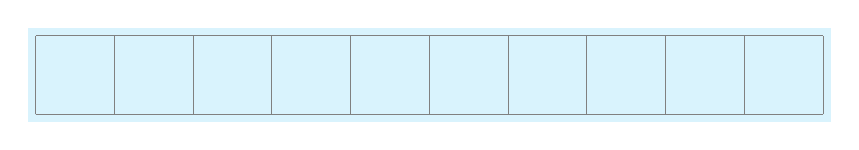
\begin{tikzpicture}
    \fill[fill=cyan!15!white] (-0.1, -0.1) rectangle (10.1, 1.1);
    \draw[step=1cm,gray,very thin] (0,0) grid (10,1);
  \end{tikzpicture}
  \caption{10 empty square strip}  
  \label{fig:empty square strip}
\end{figure}

Once our monkey will receive this strip, it will start from the left-most square --we will call this square number 1-- and will repeat the same actions according to what it sees on the spot:

\begin{enumerate}
  \item If it sees a full black square, it stops and asks for a reward
  \item If the square is empty, it either advances to the next square or, if the current one is the last one, it just stops after which it also gets a reward
\end{enumerate}

Could this situation be of any use? Not quite, but you could do one thing: having a stopwatch, you could time how long it takes for the monkey to reach an end condition. Basically, once you hand in a strip to the monkey, you would start timing and stop it once the monkey has reached a halt condition (either it got to a filled square or it ran out of strip to inspect). This might still be unusefull, but it would be a fun thing to do nonetheless.

Let's follow a quick and easy example. Suppose our strip looks as figure \ref{fig:simple example strip}.

\begin{figure}[h]
  \centering
  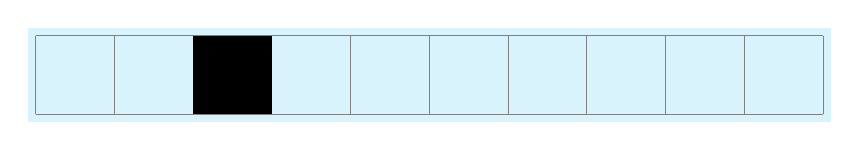
\begin{tikzpicture}
    \fill[fill=cyan!15!white] (-0.1, -0.1) rectangle (10.1, 1.1);
    \draw[step=1cm,gray,very thin] (0,0) grid (10,1);
    \fill[fill=black] (2, 0) rectangle (3, 1);
  \end{tikzpicture}
  \caption{3\textsuperscript{rd} position black-filled square strip}  
  \label{fig:simple example strip}
\end{figure}

Once our friend receives this line it will do as it was tought: it will take it, start from the leftmost square, inspect it and, if the current square is not the black one, it will advance to the next one. Of course, once it will reach the black square, it will stop.

Believe it or not, but this behavior is, at its core, very similar to what
happens in a normal computer. We \textbf{tought} our monkey, and our monkey, depending on what strip it receives, follows what we tought it to do.

How could we make this situation more usefull? you ask. Let's try doing the next thing: we all know what an "intelligent" light is. It's that light that, normally stays off, but once you go pass it, it springs to life for a few minutes before going back to sleep in preparation for the next motion to be sensed.

Needles to say, this is a good way both to extend the life of the light bulb and to save some money on the electricity bill.

We can use our clever little monkey to behave like this, but we will have to work on its knowledge a little bit. Imagine that once it receives the strip it actually turns on a switch that, in turn, lights up the environment through a light bulb. It then goes up with its normal routine and once it reaches either the end of the strip or a black-filled square, it turns off the switch, "killing" the light in the process.

This behaves in a similar manner to a an "intelligent" lighting solution if we take into consideration the fact that each action of "inspect the current square" followed by a "move to the next one", takes some time to accomplish. Basically, the light will stay on for the duration of the entire process guaranteeing that it will close eventually.

For a more intuitive feeling of this example, let's suppose that each inspecting of a square followed by the moving to a new one takes $\Delta t=3s$. For the previous strip (figure \ref{fig:simple example strip}), this will give the light bulb a total on time of roughly $2 \times \Delta t=2 \times 3s=6s$ since our monkey will inspect and advance twice before stopping. 

If, insted, we give it another strip (figure \ref{fig:second-simple example strip}), the light will stay on for $4 \times \Delta t = 4 \times 3 = 12s$.

\begin{figure}[h]
  \centering
  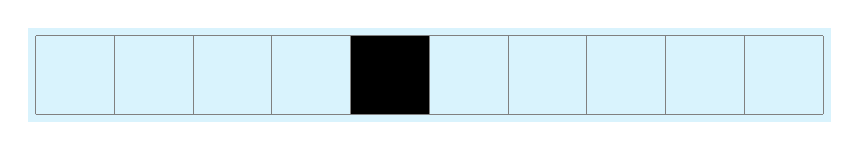
\begin{tikzpicture}
    \fill[fill=cyan!15!white] (-0.1, -0.1) rectangle (10.1, 1.1);
    \draw[step=1cm,gray,very thin] (0,0) grid (10,1);
    \fill[fill=black] (4, 0) rectangle (5, 1);
  \end{tikzpicture}
  \caption{5\textsuperscript{rd} position black-filled square strip}  
  \label{fig:second-simple example strip}
\end{figure}

From these 2 simple examples, it becomes immediatly obvious that for a longer on period, one only has to give our monkey a strip with the filled square situated on the calculated position. In other words, once tought the procedure, we can \textbf{modify its behaviour} simply by constructing a strip that fits our expected result.

If we keep the knowledge fixed --which is the easiest thing to do under these conditions--, we can only influence the end result! This is also present in the computer domain: once such machine is manufactured, it comes with a \textbf{fixed}, predefined set of symbols which it recognizes. Us, as creators, can not excede this set of symbols if we want for the computer to recognize our commands.

Having this tought behaviour, the chances for our monkey to find a working place will, for sure, increase. Because we care about our little friend's future, let's have them increased a little further.

Suppose, this time, that we manage to teach it how to recognize 4 tipes of geometrical figures, each of which triggers the execution of a particular action once it is met on the strip. Along these figures, we will also give our little friend, besides the switch that controls the initial lightbulb, one switch that controls a ringing bell and another one that controls a garage door.

These 4 primitive figures along with their interpretations are as follows:

\renewcommand{\arraystretch}{2.0}
\begin{tabular}{c m{0.75\textwidth} }
  \centering
  
\begin{tikzpicture}
    \draw[thick] (0.1, 0.1) -- (0.9, 0.1) -- (0.5, 0.9) -- cycle;
  \end{tikzpicture}
  & 
  When our monkey will meet this triangle, it will press the switch activating the ringing bell. \\
  
  
\begin{tikzpicture}
    \draw[thick] (0.1, 0.1) -- (0.9, 0.1) -- (0.1, 0.9) -- cycle;
  \end{tikzpicture}
  & 
  When it will meet this triangle, it will press the switch that opens the garage door. \\

  
\begin{tikzpicture}
    \draw[thick] (0.5, 0.1) -- (0.9, 0.5) -- (0.5, 0.9) -- (0.1, 0.5) -- cycle;
  \end{tikzpicture}
  & 
  This figure will tell our furry little friend to wait 2 minutes before carrying on with the rest of the strip (if any). \\

  
\begin{tikzpicture}
    \draw[thick] (0, 0) rectangle (1, 1);
  \end{tikzpicture}
  & 
  A square has the same interpretation as previously stated with the addition that, before stopping, it will close all the switches that it opened so far. \\
\end{tabular}
\renewcommand{\arraystretch}{1.0}

Having this extended vocabulary, we can think of even more complex and usefull tasks for our friend to accomplish. One such list could be the following:
\begin{enumerate}
\item Turn on the ringing bell 
\item Open garage door
\item Wait for 6 minutes
\item End the sequence and close all previously opened switches
\end{enumerate}

This could very well help us in building an "inteligent" garage door opener. The bell is used to alert the passing traffic that we are planning to exit or enter the premises. 

The strip required to accomplish this behavior is thus the following (see figure \ref{fig:monkey garage door openner}).

\begin{figure}[h]
  \centering
  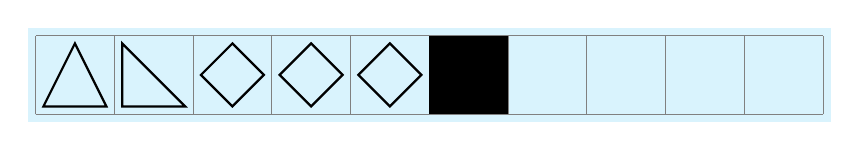
\begin{tikzpicture}
    % draw the strip grid
    \fill[fill=cyan!15!white] (-0.1, -0.1) rectangle (10.1, 1.1);
    \draw[step=1cm,gray,very thin] (0,0) grid (10,1);
    
    % add in the actions
    \draw[thick] (0.1, 0.1) -- (0.9, 0.1) -- (0.5, 0.9) -- cycle;
    \draw[thick] (1.1, 0.1) -- (1.9, 0.1) -- (1.1, 0.9) -- cycle;
    \draw[thick] (2.5, 0.1) -- (2.9, 0.5) -- (2.5, 0.9) -- (2.1, 0.5) -- cycle;
    \draw[thick] (3.5, 0.1) -- (3.9, 0.5) -- (3.5, 0.9) -- (3.1, 0.5) -- cycle;
    \draw[thick] (4.5, 0.1) -- (4.9, 0.5) -- (4.5, 0.9) -- (4.1, 0.5) -- cycle;
    \fill[fill=black] (5, 0) rectangle (6, 1);
  \end{tikzpicture}
  \caption{Garage openner strip}  
  \label{fig:monkey garage door openner}
\end{figure}

Please notice that the monkey still takes some time to read the current figure and to advance to the next one so the overall delay will not be that of $3 \times 2 minutes=6$\  minutes but, in fact, it will be closer to $3 \times 2 minutes + 3 \times \Delta t=6$\ minutes and 6 seconds. Nevertheless, for our given situation, it will have to suffice. 

\InsertImportantMark{
  Having more symbols and available actions at our disposal, the scenarios that we can solve have also increased. The total number of situations that can be tackled is therefore limited by both the number of symbols that are at our disposal and by the total placeholders supported by our strip.
}
\InsertToDo{Make an exercise that asks the reader how many scenarios can we actually generate from our given situation.}

Do you see the power of this? If, for instance, I have a garage door motor that is a little bit lazy such that 6 minutes will not suffice to fully open it and get my car in or out, we could just add in more "2 minute delay" symbols. You have to remember that we obtain this behavior just by modifying the strip. We do not touch the monkey's knowledge!

Although this can be tunned to satisfy the operation of a garage door just by sheer timing alone, it is a known fact that electrical motors degrade over time. This means that eventually, we will have to increase that wait time if we don't want to spend money on some new gear.

The problem with this approach is that, having a limited strip length which supports a fixed amount of instructions, this approach will eventually not work. In its current form, we can obtain at most 14 minutes given by using 7 delays of 2 minutes each. And that's all we can do! If we require for a delay greater then that (if we have problems with the parking, for instance), we're in serious trouble!

Let's try to fix that. We could do something like this: we could have a pressure switch being placed in the garage and use it as a way of checking whether or not the car has entered or left the premises.

To accomplish this, we need to have our little monkey learn two more symbols:

\renewcommand{\arraystretch}{2.0}
\begin{tabular}{c m{0.75\textwidth} }
  \centering
  
\begin{tikzpicture}
    \filldraw[thick] (0.5, 0.5) circle (0.2cm);
  \end{tikzpicture}
  & 
  Once our friend sees this filled circle, it will write the current state of the garage (empty or with car present). \\  
  
  
\begin{tikzpicture}
    \draw[ultra thick,red,dashed] (0.5, 0.5) circle (0.6cm);
  \end{tikzpicture}
  & 
  When our friend sees this circle drawn over one of the figures: "ring bell", "open garage door" or "delay 1 minute", it will do that action as long as the state of the garage is not different from the recorded one.\\
\end{tabular}
\renewcommand{\arraystretch}{1.0}

The sequence of instructions that our monkey will have to follow thus becomes:
\begin{enumerate}
 \item Record the current state of the garage (empty or with car)
 \item Switch on the ringing bell
 \item Switch on the garage door
 \item Delay for 2 minutes while garage state remains the same
 \item Finish the sequence of actions and close every switch
\end{enumerate}

These easily translate into the strip depicted in figure \ref{fig:monkey efficient garage door openner}. 

\begin{figure}[h]
  \centering
  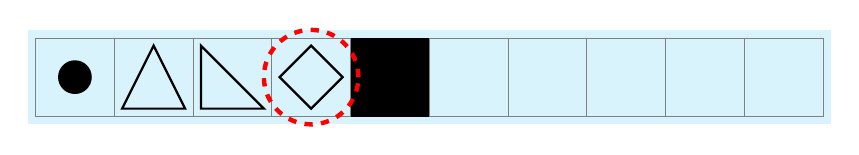
\begin{tikzpicture}
    % draw the strip grid
    \fill[fill=cyan!15!white] (-0.1, -0.1) rectangle (10.1, 1.1);
    \draw[step=1cm,gray,very thin] (0,0) grid (10,1);
    
    % add in the actions
    \filldraw[thick] (0.5, 0.5) circle (0.2cm);
    \draw[thick] (1.1, 0.1) -- (1.9, 0.1) -- (1.5, 0.9) -- cycle;
    \draw[thick] (2.1, 0.1) -- (2.9, 0.1) -- (2.1, 0.9) -- cycle;
    \draw[thick] (3.5, 0.1) -- (3.9, 0.5) -- (3.5, 0.9) -- (3.1, 0.5) -- cycle;
    \fill[fill=black] (4, 0) rectangle (5, 1);
    \draw[ultra thick,red, dashed] (3.5, 0.5) circle (0.6cm);
  \end{tikzpicture}
  \caption{Efficient garage openner strip}  
  \label{fig:monkey efficient garage door openner}
\end{figure}

There are three important things that we have to be aware of here:
\begin{enumerate}
  \item This strip version is more efficient as a garage-door openner then the previous one because it actually checks for the car before ending the procedure
  \item We manage to gain this increase in performange with a reduction of the symbol count used. This gives room for other symbols to be added on the strip if required
  \item The reduction of the symbols came at a price: some of the actions increased in complexity, meaning that our monkey had to do a quite dificult task of actually recording the state of the garage (maybe by writing it down with a pen and paper) and continuously verifying the state of the room before ending the job. 
\end{enumerate} 

\InsertToDo{Exercise: What is the difference between the previous solution and the one in which our monkey friend keeps pressing the garage-door openner switch as long as the garage state remains the same?}

The latest symbols that we tought our little companion are part of a class of tokens called \textbf{control instructions}. They form a very powerful concept which allows us to assemble complex scenarios.

Having this skill and knowing so many symbols and actions, we can safelly say that our friend's chances of geting employed have increased significantly. You know what they say : "The sounder the knowledge, the better the salary!".

On the other hand, lets suppose that I'm an employer on the lookout of a control mechanism for my garage door. Ok, I have my little monkey at my disposal but immediately I begin asking myself if there isn't a more efficient way of doing this. A way that wouldn't require so many bananas, for instance. Not surprising for anyone, there are alternatives \ldots

\section{The big step}

After all this talk about the similarities between our monkey and a computer, the next sensible thing to do is to replace our biological friend with its electronic equivalent. This way we could benefit from their obedience and efficiency without having to spend any money on physical rewards apart from electricity.

Let's start by trying to give a proper definition of what a computer might be. For a better understanding, we will make references to our monkey example use case. So, we could say that \textbf{computers are a certain type of tools (like our monkey was) that can be instructed or programmed (similar the way we taught our friend) to execute a series of ordered instructions (similar to our strip of geometrical figures) in order to obtain a desired behavior (the substitution of an "intelligent" light bulb, for instance)}.

In other words, a computer is, as are many other inventions created by humanity, a programmable machine that can do actions which have the potential of making our lives easier. The strength of these devices comes from the very fact that they can be taught. If a flash light or a mouse have fixed purposes in life, a computer can have many such scopes. We use computers to play, to work, to organize our lives and many-many more other things, all from the comfort of a single tool.

Table \ref{tab:monkey-computer similarities} synthesizes the features that are common to both our monkey universe and to the computer technical domain.

\begin{table}
  \centering
  \renewcommand{\arraystretch}{2.0}
  \begin{tabular}{| c | c |}
    \hline
    % Add the table header
    \cellcolor{blue!15}\textbf{Monkey example}
    & 
    \cellcolor{blue!15}\textbf{Computer equivalence} \\  \hline

    Our monkey itself & The computer \\ \hline
    The strip & Instruction memory \\ \hline
    The monkey's notebook & Data memory \\ \hline
    Geometrical symbols & Instructions \\ \hline
    Physical switches & Specialized internal modules \\ \hline
  \end{tabular}
  \caption{Monkey--Computer similarities}
  \label{tab:monkey-computer similarities}
  \renewcommand{\arraystretch}{1.0}
\end{table}

In the following sections we will try to go deeper with understanding and explaining these mappings, all except the first one, "monkey -- computer", since it is the one that sums up the rest of the features.

\section{Do we really math-talk to a computer?}

\ldots do we really want this? Do we really want to draw each and every time we wish to check our email? Of course not! Although it is true that we have to write symbols to tell it what to do, there is a different kind of vocabulary that we have to use. What makes this computer vocabulary special is the fact that it contains only zeroes (0) and ones (1). This is why we also say that this vocabulary forms a \textit{binary system} and that these entities are called \textit{binary values}. 

It is no coincidence that there are only 2 indivisible symbols in a computer vocabulary for they have some electrical merits as well as some logical and mathematical advantages. Logical because these 2 symbols can be interpreted, at a more fundamental level, as \textbf{true} and \textbf{false}.On the other hand, we say that it has "mathematical advantages" because we can define mathematical operations to them, reconstructing numbers and building expressions. This is something we call boolean algebra\footnote{It comes from its inventor, \InsertProperName{George Boole}, an English mathematician who lived in the \textsc{XIX}\textsuperscript{th} century.} 

Using only these 2 elements, we as computer instructors better known as computer programmers, can construct long sequences of unique strings that tell the computer what to do. One such sequence could be the one shown in figure \ref{fig:sequence of binary elements}.

\begin{figure}[h]
  \centering
  \huge
  \textbf{010111000101101001110110001}
  \caption{Sequence of binary elements}
  \label{fig:sequence of binary elements}
\end{figure}

Uniqueness is important in this context since it guarantees that the desired action is not missinterpreted by the computer. For instance, when we talked about our monkey example, we had unique symbols that controlled individual actions. 

For clarity, lets suppose we want to encode our original geometric symbols using this new, lightweight, alphabet. Of course, we could not accomplish this just by using one symbol, therefore, we would require to have a group of such elements being interpreted as the figures themselves. The first question that we have to ask ourselves is what length should we pick for one such group element? We could just give them a variable length and add symbols when we feel the need to, but this is not elegant and it posses some serious practical problems as well. We have to settle up for a number.

Let's think \ldots\ We can encode 2 geometric symbols with one binary value since one binary value can take either value 1 or 0. With 2 binary values, we can encode 4 such physical figures since we can construct 4 unique groups: "00", "01", "10" and "11". In general, $n$ binary symbols can encode $2^n$ graphical symbols. 

We need to encode 6 symbols and a control element that can be applied to 3 of the actions, giving a total of $6 + 3 = 9$ combinations. With $n=3$ we could encode up to $2^3=8$ geometric symbols (still not enough) while choosing $n=4$ let's us encode $2^4=16$ primitives. Bingo!

We could have found the solution faster if we would have used the mathematical inverse operation for exponentiation which is applying a  logarithm. In our case, the solution would have been obtained fairly straightforward: $\lceil \log_2 9 \rceil = \lceil 3.169 \rceil = 4$.

Having the length of the binary group, we can move on and assign an arbitrary value to each of the known symbols. One such solution could be that described in table \ref{tab:binary-graphical encoding}.

\begin{table}[h]
  \centering
  \renewcommand{\arraystretch}{2.46}
  \begin{tabular}{| c | c |}
    \hline
    % Add the table header
    \cellcolor{blue!15}\textbf{Graphical symbol}
    & 
    \cellcolor{blue!15}\textbf{Binary proposed encoding} \\  \hline

    
\begin{tikzpicture}[baseline]
      \draw[thick] (-0.25, -0.25) rectangle (0.75, 0.75);
    \end{tikzpicture}
    & 
    {\large 0000} \\ \hline

    
\begin{tikzpicture}[baseline]
      \draw[thick] (-0.2, -0.2) -- (0.6, -0.2) -- (0.2, 0.6) -- cycle;
    \end{tikzpicture}  
    & 
    {\large 0001} \\ \hline

    
\begin{tikzpicture}[baseline]
      \draw[thick] (0.2, -0.2) -- (0.6, 0.2) -- (0.2, 0.6) -- (-0.2, 0.2) -- cycle;
    \end{tikzpicture}
    & 
    {\large 0010} \\ \hline

    
\begin{tikzpicture}[baseline]
      \draw[thick] (-0.2, -0.2) -- (0.6, -0.2) -- (-0.2, 0.6) -- cycle;
    \end{tikzpicture}
    &
    {\large 0011} \\ \hline
    
    
\begin{tikzpicture}[baseline]
      \filldraw[black] (-0.25, -0.25) rectangle (0.75, 0.75);
    \end{tikzpicture}
    &
    {\large 0100} \\ \hline
    
    
\begin{tikzpicture}[baseline]
      \filldraw[black] (0.2, 0.2) circle (0.2cm);
    \end{tikzpicture}
    &
    {\large 0101} \\ \hline \hline
    
    % 'control specifier' region
    
\begin{tikzpicture}[baseline]
      \draw[thick] (-0.2, -0.1) -- (0.6, -0.1) -- (0.2, 0.7) -- cycle;
      \draw[ultra thick,red,dashed] (0.2, 0.2) circle (0.6cm);
    \end{tikzpicture}
    &
    {\large 1001} \\ \hline
    
    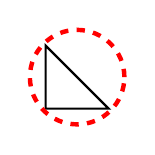
\begin{tikzpicture}[baseline]
      \draw[thick] (-0.2, -0.2) -- (0.6, -0.2) -- (-0.2, 0.6) -- cycle;
      \draw[ultra thick,red,dashed] (0.2, 0.2) circle (0.6cm);
    \end{tikzpicture}
    &
    {\large 1010} \\ \hline
    
    
\begin{tikzpicture}[baseline]
      \draw[thick] (0.2, -0.2) -- (0.6, 0.2) -- (0.2, 0.6) -- (-0.2, 0.2) -- cycle;
      \draw[ultra thick,red,dashed] (0.2, 0.2) circle (0.6cm);
    \end{tikzpicture}
    &
    {\large 1011} \\ \hline
  \end{tabular}
  \caption{Variant encoding of graphical symbols using binary groups}
  \label{tab:binary-graphical encoding}
  \renewcommand{\arraystretch}{1.0}
\end{table}

If you look carefully, you will see that the table is in fact split in half. On the one side you have the normal, un-circled instructions while on the lower half you have your control specifier applied to its 3 supported instructions. This is necessary since the specifier itself doesn't have any meaning of its own and has to be groupped with another element for this to happen.

The suggested variant encapsulates two good design principles for such activities: 
\begin{enumerate}
  \item It assigns the "all-zero" group to the symbol that dictates no effect -the empty square-. This might be a strange thing to do at first but does bring engineering benefits to the computer designer. It might help to think that it's much easy to say that "the do-nothing symbol has all zeroes" than "the do-nothing symbol has 1011".
  \item It encodes the control specifier as the leftmost binary symbol in the encoding. In other words, if you compare the lower half symbol encodings with their originals, you will notice that they have the 3 rightmost characters the same and only differ in the last, leftmost value: a "1" signals that the control specifier was added while a "0" signals the lack of it. This makes the encoding both easy to extend and to memorise and  recognise both by the humans and by the computer itself.
\end{enumerate}

After encoding the symbols and making them available for a computer environment, we can go on and rewrite the equivalent "strip". This will allow the machine to follow, interpret and execute the sequence, obtaining the same end-result as our little monkey did. We accomplish this in figure \ref{fig:garage binary strip}.

\begin{figure}[h]
  \centering  
  \begin{tabular}{c | c | c | c | c | c | c | c | c | c}
    {\large 0101} & 
    {\large 0001} & 
    {\large 0011} & 
    {\large 1011} &
    {\large 0100} &
    {\large 0000} &
    {\large 0000} &
    {\large 0000} &
    {\large 0000} &
    {\large 0000} \\
  \end{tabular}
  \caption{Binary strip for the garage door openner problem}
  \label{fig:garage binary strip}
\end{figure}

Of course, this is a control problem requiring a control solution, but how could we use this simple vocabulary for more practical, numerical formulations? How could we use the binary system to represent real-world numbers?

One solution might be to start from the symbols of the \textit{decimal system} --the one we use so often in our day-to-day lives-- and have each of them mapped to a unique group of binary values. 

There are 10 decimal symbols which implies that the binary group has a length of $\lceil \log_2 10 \rceil = \lceil 3.321 \rceil = 4$ symbols. One such mapping could be that portrayed in figure \ref{fig:binary-decimal initial mapping}.

\begin{figure}[h]
  \centering
  \renewcommand{\arraystretch}{1.5}
  \begin{tabular}{c | c | c | c | c | c | c | c | c | c}
    {\Large 0} & {\Large 1} & {\Large 2} & {\Large 3} & {\Large 4} & {\Large 5} & {\Large 6} & {\Large 7} & {\Large 8} & {\Large 9} \\ \hline
    {\large 0000} & {\large 0001} & {\large 0010} & {\large 0011} & {\large 0100} & {\large 0101} & {\large 0110} & {\large 0111} & {\large 1000} & {\large 1001} \\
  \end{tabular}
  \renewcommand{\arraystretch}{1.0}
  \caption{Proposed binary $\leftrightarrow$ decimal symbol mapping}
  \label{fig:binary-decimal initial mapping}
\end{figure}

Having this, we could go on and directly convert each decimal digit from a number to its 4 group equivalence. Let's take an example: Let's say we have  the number 18301 to which we want to find its binary equivalance using figure \ref{fig:binary-decimal initial mapping}. Simple enough, we only have to extract the decimal digits and find their respectfull binary group. Figure \ref{fig:binary-decimal 18301 example} shows this process happening.

\begin{figure}[h]
  \centering
  \renewcommand{\arraystretch}{1.5}
  \begin{tabular}{c c c c c}
    {\Large 1} & {\Large 8} & {\Large 3} & {\Large 0} & {\Large 1} \\ \hline
    {\large 0001} & {\large 1000} & {\large 0011} & {\large 0000} & {\large 0001} \\
  \end{tabular}
  \renewcommand{\arraystretch}{1.0}
  \caption{Decimal $\leftrightarrow$ binary of "18301"}
  \label{fig:binary-decimal 18301 example}
\end{figure}

Although this approach seems a sane one, it has its drawbacks which makes it hardly usable:

\begin{itemize}
  \item It requires a fixed count of 4 binary elements per digit which consumes a lot of memory.
  \item The encoding is not that very efficient. From the $2^4=16$ unique combinations that can be obtained using a 4 binary group, only 10 values are used generating a waste of $\frac{6}{16} \times 100 = 37.5\%$. This is a very bad value!
  \item The selected encoding, altough easy to traverse back and forth between the two systems, poses serious implementation issues for computer designers.
\end{itemize}

Clearly, we have to search for a more efficient solution that must be both more designer friendly and less wasteful in terms of unused values.

The way the people working in this domain do this is by employing a mathematical operation. Suppose we note with $B^n_i$ the i\textsuperscript{th} binary symbol from a binary group consisting of $n$ elements, $B^n_i \in \{0, 1\}$. Thus, $B^n$ can be rewritten, by definition, as a concatenation of binary elements as shown by equation \ref{eq:general binary concatenation}.

\begin{equation}
  B^n=B^n_n...B^n_2B^n_1B^n_0
  \label{eq:general binary concatenation}
\end{equation} 

To find the decimal equivalency --noted $D_B$-- of binary group $B^n$, one must do the calculations described by equation \ref{eq:binary to decimal calc. algo.}.

\begin{equation}
  D_B=\sum^n_{i=0}(B^n_i \times 2^i)
  \label{eq:binary to decimal calc. algo.}
\end{equation}

Lets apply this formula for an example to better understand its operation. Suppose we have the following binary group (figure \ref{fig:binary to decimal 11001 example}) for which we want to calculate its decimal value according to equation \ref{eq:binary to decimal calc. algo.}.

\begin{figure}[h]
  \centering
  \renewcommand{\arraystretch}{1.5}
  \begin{tabular}{c c c c c}
    {\Large 1} & {\Large 1} & {\Large 0} & {\Large 0} & {\Large 1} \\
  \end{tabular}
  \renewcommand{\arraystretch}{1.0}
  \caption{Example of binary group to be converted to its decimal value}
  \label{fig:binary to decimal 11001 example}
\end{figure}

First we observe that the group has 5 binary elements thus making $n=5$. Going forward and applying the conversion formula, we unroll the group as fallows (figure \ref{fig:binary to decimal 11001 example adnoted}). 

\begin{figure}[h]
  \centering
  \renewcommand{\arraystretch}{1.5}
  \begin{tabular}{c c c c c}
    {\small 4} & {\small 3} & {\small 2} & {\small 1} & {\small 0} \\ \hline
    
    {\cellcolor{blue!05}\Large 1} & 
    {\cellcolor{blue!05}\Large 1} & 
    {\cellcolor{blue!05}\Large 0} & 
    {\cellcolor{blue!05}\Large 0} & 
    {\cellcolor{blue!05}\Large 1} \\ \hline
    
    $B^4_4$ & $B^4_3$ & $B^4_2$ & $B^4_1$ & $B^4_0$ \\
  \end{tabular}
  \renewcommand{\arraystretch}{1.0}
  \caption{Further details to the 11001 conversion example}
  \label{fig:binary to decimal 11001 example adnoted}
\end{figure}

Applying the aforementioned conversion formula, we obtain: $\sum_{i=0}^4(B^4_i \times 2^i) = B^4_0 \times 2^0 + B^4_1 \times 2^1 + B^4_2 \times 2^2 + B^4_3 \times 2^3 + B^4_4 \times 2^4 = 1 \times 2^0 + 0 \times 2^1 + 0 \times 2^2 + 1 \times 2^3 + 1 \times 2^4 = 2^0 + 2^3 + 2^4 = 1 + 8 + 16 = 25$.

On the other hand, going from decimal to binary, the process is a little bit more different. While to obtain a decimal equivalence one has to sum up some terms, the roundtrip will require a decomposition of some sort.

The rule that we will need to apply in order to obtain the binary equivalence of a decimal value, is given by the pseudocode from listing \ref{cod:decimal-to-binary pseudocode}.

\begin{pseudocode}[caption={Decimal to binary conversion algorithm}, label={cod:decimal-to-binary pseudocode}]
  $\textbf{Input}$  : N $\equiv$ Decimal value which we want converted  
  $\textbf{Output}$ : B $\equiv$ List of binary symbols that form N
  
  B $\leftarrow$ ()
  while N $\not =$ 0
    Push in front of list B the result of (N mod 2)
    N $\leftarrow \lfloor n \div 2 \rfloor$ 
  end  
  return B
\end{pseudocode}

Taking up an example will likely to make things easier to understand. Let's suppose we want to convert the decimal value "37" to its binary equivalence. Applying the procedure from listing \ref{cod:decimal-to-binary pseudocode}, we obtain the results captured in listing \ref{cod:37 decimal-to-binary pseudocode example}.

\begin{figure}[h]
  \begin{pseudocode}[caption={"37" decimal-to-binary conversion example}, label={cod:37 decimal-to-binary pseudocode example}]
  N $\leftarrow$ 37; B $\leftarrow$ ()
  37 $\not =$ 0 (T) $\Rightarrow$ B $\leftarrow$ (1 [= 37 mod 2]), N $\leftarrow \lfloor 37 \div 2 \rfloor$ = 18
  18 $\not =$ 0 (T) $\Rightarrow$ B $\leftarrow$ (0 [= 18 mod 2], 1), N $\leftarrow \lfloor 18 \div 2 \rfloor$ = 9
  9 $\not =$ 0 (T) $\Rightarrow$ B $\leftarrow$ (1 [= 9 mod 2], 0, 1), N $\leftarrow \lfloor 9 \div 2 \rfloor$ = 4
  4 $\not =$ 0 (T) $\Rightarrow$ B $\leftarrow$ (0 [= 4 mod 2], 1, 0, 1), N $\leftarrow \lfloor 4 \div 2 \rfloor$ = 2
  2 $\not =$ 0 (T) $\Rightarrow$ B $\leftarrow$ (0 [= 2 mod 2], 0, 1, 0, 1), N $\leftarrow \lfloor 2 \div 2 \rfloor$ = 1
  1 $\not =$ 0 (T) $\Rightarrow$ B $\leftarrow$ (1 [= 1 mod 2], 0, 0, 1, 0, 1), N $\leftarrow \lfloor 1 \div 2 \rfloor$ = 0
  0 $\not =$ 0 (F) $\Rightarrow$ return B $\Rightarrow$ (1, 0, 0, 1, 0, 1) = 100101
  \end{pseudocode}
\end{figure}

Basically, we started of with 37 and divided repeatedly keeping track of the reminder. Once there was nothing more to devide ($N=0$), the result was basically the reminders returned in reverse order in which they were obtained. To verify that this binary group --100101-- is actually the correct result, I advice you to try to convert this group back to the decimal value using the method previously discussed.

One of the advantages of using these conversion methods solves the efficiency problem in the sense that no binary symbols are waisted. By having this approach, a higher degree of values can be represented using a low number of binary symbols. For instance, having a group of 32 binary symbols, we can represent 4294967296 unique decimal values!

Although this variant is more efficient in terms of value coverage and computer design considerations --making it easy for implementing mathematical operations in hardware--, this does come at a price: numbers expressed in this fashion are impossible to quickly decypher with the naked eye alone. While this is not so much of a problem for modern day computers and their easy to follow, sofisticated programming languages, when the first computers apeared the programmers didn't have such modern tools to rely on. The first computers were programmed at a binary level therefore making the need for a compact representation even more important and urgent for productivity reasons.

One way of solving this interpretation situation is to still use the first representation, but to try to assign usefull symbols for the rest of the unused binary groups. A question then arises: What shall the remaining binary values represent? We consumed all the 10 symbols from the decimal system and we have 6 more placeholders available. It would be nice to have them cover a 16 symbol numerical system. As it is the case in mathematics, such a system exists and it is called a \textit{hexadecimal system} or \textit{hex}, for short.

The hexadecimal system contains the following symbols (figure \ref{fig:hex symbols}). To quickly convert such a 4 symbol binary group to and from this numerical system, you would only need to search its equivalence in figure \ref{fig:binary-hex complete mapping}. 

\begin{figure}[h]
  \centering
  \huge
  \textbf{0 1 2 3 4 5 6 7 8 9 A B C D E F}
  \caption{Hex symbols}
  \label{fig:hex symbols}
\end{figure}

\begin{figure}[h]
  \centering
  \renewcommand{\arraystretch}{1.5}
  % 0-9 values
  \begin{tabular}{c | c | c | c | c | c | c | c | c | c}
    {\Large 0} & {\Large 1} & {\Large 2} & {\Large 3} & {\Large 4} & {\Large 5} & {\Large 6} & {\Large 7} & {\Large 8} & {\Large 9} \\ \hline
    {\large 0000} & {\large 0001} & {\large 0010} & {\large 0011} & {\large 0100} & {\large 0101} & {\large 0110} & {\large 0111} & {\large 1000} & {\large 1001} \\
  \end{tabular}
  \vspace{0.5cm}

  % A-F values  
  \begin{tabular}{ c | c | c | c | c | c }
     {\Large A} & {\Large B} & {\Large C} & {\Large D} & {\Large E} & {\Large F} \\ \hline
     {\large 1010} & {\large 1011} & {\large 1100} & {\large 1101} & {\large 1110} & {\large 1111}\\  
  \end{tabular}
  
  \renewcommand{\arraystretch}{1.0}
  \caption{Binary $\leftrightarrow$ hex symbol mapping}
  \label{fig:binary-hex complete mapping}
\end{figure}

Thus, if we wanted to find out, for example, what is the binary equivalent for the hex number 56? We would lookup the 2 symbols in the table and find out that they map to groups 0101 and 0110, leading to a unified representation of 01010110. This, of course, works also well the other way around: having to "shrink" the binary groups to their hex equivalence.

To find the decimal value of a hex number, you could accomplish this as a 2 step process:
\begin{enumerate}
  \item Find the binary value from the hex value
  \item Calculate the decimal equivalent of the binary group
\end{enumerate}
This method allows for a reverse --decimal to hex-- procedure as well.

Do you see a problem here? Being an extension to the decimal symbols, this becomes a source of confusion. For instance, what is the diference between "56" expressed in  decimal and "56" expresed in the hex system? They are identical the way they are written!

To resolve this issue, we have 2 solutions. The first one is to subscript the value with its base symbol count: 2 for binary, 10 for decimal and 16 for hexadecimal. Thus, 110 in decimal becomes $110_{10}$, binary has it expressed as $110_2$, while the same number written in hexadecimal is $110_{16}$.

If subscripting is not available --which is the case when we write these values using a computer--, we have the alternative of a prefix notation: \textbf{0b} for binary, \textbf{0x} for hex and a no-prefix for the more general case of decimal representations. In this situation, 110 is considered to be in decimal format, 0x110 is a hex number and 0b110 is to be interpreted as a binary group. It's worth mentioning that we will be using this way of number representation when we will comunicate with the pAle board.

Before we carry on, I think it's better to clarify the dimmension characteristic as well. We talked about groups of binary symbols having an arbitrary length $n$. In practice, due to hardware constrains, this value is fixed by the computer manufacturer. Traditionally and conventionally, $n$ was choosen to be 8, giving what is called "the atom of factual information", \textbf{a byte}. Also, computer people regard one binary symbol as being one \textbf{bit} of information.

Of course, longer groups of binary symbols (bits) are possible, but they are, by convetion and implementation, a multiple of bytes.

Having this said, I believe we have now the foundations to carry on with another interesting topic in computer behavior. We will talk next about memories \ldots

\section{Here comes the memories}


\section{What can computers do?}
\section{When two universes colide}
\chapter{Here comes she}
\section{Ale is a thinker}
\subsection{Her memory}
\subsection{Her vocabulary}
\section{A small talk about Attiny25's modules}

\part[The Present]{The Present\\[2ex]\makebox[0pt]{
      \includegraphics[scale=0.3]{./img/altele/deschidere_partea2.jpg}
  }
}

\chapter{Ale meets the world}
\section{[1s]Ale, do nothing!}
\section{[2s]Ale's general register load-up}
\section{[3s]Ale says 'Hi!'}
\section{[4s]Ale says a better 'Hi!'}
\section{[4.1s]A proof of Ale's thinking}
\section{[5s]Slow down Ale!}
\section{[5.1s]Where is the stack?}
\section{[6s]Two nice LED example}
\section{[7s]We are here Ale!}
\section{[8s]We are still here Ale!}
\section{[9s]If all is Ok, let's carry on}
\section{[10s]Better delays}
\section{[11s]No interruptions, please!}
\section{[12s]Another interrupt, same timer0}
\section{[12.1s]Watch out for interrupts!}
\section{[13s]Interrupts yet again}
\section{[14s]When one is not enough}
\section{[15s]When miliseconds are not enough}
\section{[16s]A more able clock}
\section{[17s]Together onto wonderful things}
\section{[18s]Our best friend, the watchdog}
\section{[19s]Who reseted me, I wonder?}
\section{[20s]Eco Ale!}
\section{[21s]A psAle and a Ale. Hi Ale!}
\section{[22s]What's the temperature, Ale?}
\section{[23s]Ale doesn't need glasses}
\section{[24s]Back from where we started}
\subsection{[G1]PIG}
\subsection{[G2]36}
\chapter{Something different}
\section{Less code is a beautiful code}
\section{Here comes the C}

\part[The Horizon]{The Horizon\\[2ex]\makebox[0pt]{
      \includegraphics[scale=1.5]{./img/altele/deschidere_partea3.jpg}
  }
}

\chapter{Congratz! You made it}
\section{... all the way to the end!}
\section{, but the game must go on}
\chapter{Extensoes}
\section{psAle install instructions}
\section{psAle user manual}
\section{Solution variants}
\subsection{[1s]Ale, do nothing!}
\subsection{[2s]Ale's general register load-up}
\subsection{[3s]Ale says 'Hi!'}
\subsection{[4s]Ale says a better 'Hi!'}
\subsection{[4.1s]A proof of Ale's thinking}
\subsection{[5s]Slow down Ale!}
\subsection{[5.1s]Where is the stack?}
\subsection{[6s]Two nice LED example}
\subsection{[7s]We are here Ale!}
\subsection{[8s]We are still here Ale!}
\subsection{[9s]If all is Ok, let's carry on}
\subsection{[10s]Better delays}
\subsection{[11s]No interruptions, please!}
\subsection{[12s]Another interrupt, same timer0}
\subsection{[12.1s]Watch out for interrupts!}
\subsection{[13s]Interrupts yet again}
\subsection{[14s]When one is not enough} % environment used for inserting pseudocode into the document
\newenvironment{PseudoCode}{%
\begin{lstlisting}[numbers=left, framexleftmargin=5mm, frame=shadowbox, rulesepcolor=\color{blue}]}{%
\end{lstlisting}}
\subsection{[15s]When miliseconds are not enough}
\subsection{16s]A more able clock}
\subsection{[17s]Together onto wonderful things}
\subsection{[18s]Our best friend, the watchdog}
\subsection{[19s]Who reseted me, I wonder?}
\subsection{[20s]Eco Ale!}
\subsection{[21s]A psAle and a Ale. Hi Ale!}
\subsection{[22s]What's the temperature, Ale?}
\subsection{[23s]Ale doesn't need glasses}
\subsection{[24s]Back from where we started}
\section{Attiny25's register sheet}
\section{pAle's schematic}
\end{document}
